\documentclass{article}

\setlength{\headsep}{0.75 in}
\setlength{\parindent}{0 in}
\setlength{\parskip}{0.1 in}

%=====================================================
% Add PACKAGES Here (You typically would not need to):
%=====================================================

\usepackage{xcolor}
\usepackage[margin=1in]{geometry}
\usepackage{amsmath,amsthm}
\usepackage{fancyhdr}
\usepackage{enumitem}
\usepackage{graphicx}

%=====================================================
% Ignore This Part (But Do NOT Delete It:)
%=====================================================

\theoremstyle{definition}
\newtheorem{problem}{Problem}
\newtheorem*{fun}{Fun with Algorithms}
\newtheorem*{challenge}{Challenge Yourself}
\def\fline{\rule{0.75\linewidth}{0.5pt}}
\newcommand{\finishline}{\begin{center}\fline\end{center}}
\newtheorem*{solution*}{Solution}
\newenvironment{solution}{\begin{solution*}}{{\finishline} \end{solution*}}
\newcommand{\grade}[1]{\hfill{\textbf{($\mathbf{#1}$ points)}}}
\newcommand{\thisdate}{\today}
\newcommand{\thissemester}{\textbf{Rutgers: Spring 2021}}
\newcommand{\thiscourse}{CS 344: Design and Analysis of Computer Algorithms} 
\newcommand{\thishomework}{Number} 
\newcommand{\thisname}{Name} 
\newcommand{\thisextension}{Yes/No} 

\headheight 40pt              
\headsep 10pt
\renewcommand{\headrulewidth}{0pt}
\lhead{\small \textbf{Only for the personal use of students registered in CS 344, Spring 2021 at Rutgers University. Redistribution out of this class is strictly prohibited.}}
\pagestyle{fancy}

\newcommand{\thisheading}{
   \noindent
   \begin{center}
   \framebox{
      \vbox{\vspace{2mm}
    \hbox to 6.28in { \textbf{\thiscourse \hfill \thissemester} }
       \vspace{4mm}
       \hbox to 6.28in { {\Large \hfill Homework \#\thishomework \hfill} }
       \vspace{2mm}
         \hbox to 6.28in { { \hfill \thisdate  \hfill} }
       \vspace{2mm}
       \hbox to 6.28in { \emph{Name: \thisname \hfill Extension: \thisextension}}
      \vspace{2mm}}
      }
   \end{center}
   \bigskip
}

%=====================================================
% Some useful MACROS (you can define your own in the same exact way also)
%=====================================================


\newcommand{\ceil}[1]{{\left\lceil{#1}\right\rceil}}
\newcommand{\floor}[1]{{\left\lfloor{#1}\right\rfloor}}
\newcommand{\prob}[1]{\Pr\paren{#1}}
\newcommand{\expect}[1]{\Exp\bracket{#1}}
\newcommand{\var}[1]{\textnormal{Var}\bracket{#1}}
\newcommand{\set}[1]{\ensuremath{\left\{ #1 \right\}}}
\newcommand{\poly}{\mbox{\rm poly}}


%=====================================================
% Fill Out This Part With Your Own Information:
%=====================================================


\renewcommand{\thishomework}{4} %Homework number
\renewcommand{\thisname}{Letao Zhang} % Enter your name here
\renewcommand{\thisextension}{Yes} % Pick only one of the two options accordingly

\begin{document}

\thisheading
\vspace{-0.75cm}


%=====================================================
% LaTeX Tip: You can erase this part from here.... 
%=====================================================		

\subsection*{Homework Policy}
\begin{itemize}
\item If you leave a question completely blank, you will receive 25\% of the grade for that question. This however does not apply to the extra credit questions.
\item You are allowed to discuss the homework problems with other students in the class. \textbf{But you must write your solutions independently.} 
You may also consult all the materials used in this course (video recordings, notes, textbook, etc.) while writing your solution, but no other resources are allowed.
\item Do not forget to write down your name and whether or not you are using one of your two extensions. Submit your homework on Canvas. 
\item Unless  specified otherwise, you may use any algorithm covered in class as a ``black box'' -- for example you can simply write ``use Prim's or Kruskal's algorithm to find an MST of the input graph in $O(m\log{m})$ time''. 
You are \textbf{strongly encouraged to use graph reductions} instead of designing an algorithm from scratch whenever possible (even when the question does not ask you to do so explicitly). 

\item Remember to always \textbf{prove the correctness} of your algorithms and \textbf{analyze their running time} (or any other efficiency measure asked in the question). 

\item The ``Challenge yourself'' and ``Fun with algorithms''  are both extra credit. These problems are significantly more challenging than the standard problems you see in this course (including lectures, homeworks, and exams). 
As a general rule, only attempt to solve these problems if you  enjoy them. 
\end{itemize}

\finishline

\begin{problem}
You are given the map of $n$ cities with $m$ bidirectional roads between different cities. You are asked to construct airports in some of the cities such that each city either has an airport itself or there is a way to go from this city to a city with an airport 
using the given roads---moreover, you can also construct a road between any two cities if there is no road between them already. Finally, you are told that the cost of constructing an airport is $a$ and the cost of connecting any two cities 
by a new road is $r$. 

Design and analyze an $O(n+m)$ time algorithm that given the number $n$ of the cities, the $m$ roads between them, and the costs $a$ and $r$, outputs the locations of airports and roads to be constructed 
to satisfy the conditions above, while having the minimum possible cost. \grade{25}

\paragraph{Examples:}

\begin{enumerate}
    \item \emph{Input:} $n=4$ cities with $m=2$ roads $(1,2), (2,3)$, cost of constructing an airport $a = 7$, and constructing a road is $r=5$. 
    
   \emph{Output:} The minimum cost needed is 12 -- we construct an airport in city $4$ and connect it this city via a road to any of the cities $1$, $2$, or $3$ (chosen arbitrarily). 
 
    \item \emph{Input:} $n=4$ cities with $m=2$ roads $(1,2), (2,3)$, cost of constructing an airport $a = 7$, and constructing a road is $r=8$. 
    
   \emph{Output:} The minimum cost needed is 14 -- we construct an airport in city $4$ and another one in any one of the cities $1$, $2$, or $3$ (chosen arbitrarily). 

\end{enumerate}
\end{problem}

\begin{solution}
	
	\emph{Algorithm.} Simply we can use Depth-First Search(DFS) to analysis this question and find the minimum possible cost. 
	
	a) Initialize an array mark[1 : n] with ‘FALSE’. Run the following recursive algorithm on s, i.e., return DFS(s). 
	
	b) DFS(v) : 1. If mark[v] = ‘TRUE’ terminate. 2. Otherwise, set mark[v] =‘TRUE’ and for every neighbor $u \in N(v)$. 
	
	c) Then we construct at least one airport in one of the city base on the minimum cost. 
	
	At the end, we return all vertices v with mark[v] = ‘TRUE’ as the answer, i.e., as vertices that are in the same connected component of s. \\

	\emph{Proof of Correctness.} We need to prove that every vertex connected to s will be output and no other vertex is also output by this algorithm. The second part is straightforward because we are only visiting s, neighbors of s, their neighbors and so on and so forth, so for any vertex marked, there is a path from s to that vertex in the graph. The other part is also easy: consider any unmarked vertex u. We prove that u is not in the connected component of s. Since u is unmarked, none of the neighbors v of u can be marked: otherwise, when we visited v for the first time, we would have marked u also at some point later. We can then continue like this to all neighbors of v and say that all neighbors of v needs to be unmarked also. We expand this until we find all of the vertices that are connected to u and we know that they are all unmarked. But this means that s was not any of those vertices since s is actually marked; hence u cannot be part of the connected component of s since there is no path from s to u. \\
	
	\emph{Runtime Analysis.} The runtime is same as the runtime for DFS that we visit each vertex v at most once (after that it is marked and we do not spend more time in visiting the vertex (think of memoization)) and it takes $O(\left| N(v) \right|)$ time to process this vertex. Hence, the total runtime is at most $c · \sum _{v \in V} |N(v)|$ for some constant c: since the total degree of vertices is proportional to the number of edges, the runtime of this algorithm is $O(n + m)$.


\end{solution}



\begin{problem}
	We say that an undirected graph $G=(V,E)$ is \textbf{$2$-edge-connected} if we need to remove \emph{at least two} edges from $G$ to make it disconnected. Prove that a 
	graph $G=(V,E)$ is $2$-edge-connected if and only if for every cut $(S,V-S)$ in $G$, there are \emph{at least two cut edges}, i.e., $|{\delta(S)}| \geq 2$. \grade{25}
\end{problem}


\medskip

\begin{solution}

	1) Similarly, a graph is k-edge connected if it has at least two vertices and no set of $k-1$ edges is a separator. If it is a 2-edge-connected graph, then every edge is in a cycle. 
	
	2) If G is connected then every cut in G has at least one cut edge. We prove this by contradiction. Suppose G is connected but there exists a cut (S, V - S) with $|\delta(S)| = 0$. Pick any vertex u in S and any vertex v in $V-S$. Since G is connected, there should be path from u to v in G. Let us say the path is P = u, w1, w2, . . . , wk, v. Find the first index i such that $wi \in S and wi+1 \in V - S$; such an index should exists because $u \in S$ and $v \in V - S$ and so along this path we should eventually move from S-part to $(V - S)$-part. But now the edge $(w_i, w_i+1)$ is a cut edge of S, a contradiction. 

	3) If there is no cutset and G has at least two vertices, we say G has connectivity $n-1$; if G has one vertex, its connectivity is undefined. If G is not connected, we say it has connectivity 0. G is k-connected if the connectivity of G is at least k. The connectivity of is denoted K(G). 

	4) Therefore, we know that any 2-edge-connected graph $G=(V,E)$ is connected if and only if every cut $(S,V-S)$ in G has at least two cut edge, namely, $|{\delta(S)}| \geq 2$ for all $S \subset V$. \\
	
\end{solution}


\medskip

\begin{problem}
	The Muddy City consists of $n$ houses but no proper streets; instead, the different houses are connected to each other via $m$ bidirectional muddy roads. The newly elected mayor of the city aims to pave some of these roads to ease
	the travel inside the city but also does not want to spend too much money on this project, as paving each road $e$ between houses $u$ and $v$ has a certain cost $c_e$ (different across the muddy roads). The mayor thus specifies two conditions: 
	\begin{itemize}
		\item Enough streets must be paved so that everyone can travel from any house to another one using only the paved roads (you may assume that this is always possible); 
		\item The paving should cost as little as possible. 
	\end{itemize}
	You are chosen to help the mayor in this endeavor.  
	
	\begin{enumerate}
		\item [(a)] Design and analyze an $O(m\log{m})$ time algorithm for this problem. \grade{10} 
		
		\medskip

\begin{solution}

	\emph{Algorithm.} We are using Minimum Spanning Tree (MST) to pave some of these roads using minimum cost. Using Kruskal’s algorithm with union-find data structure works as follows: 
	
	1) Sort the edges of G in increasing (non-decreasing) order of their weights. 2) Create a union-find data structure D with preprocess(n) (with universe $U = {v_1, . . . , v_n}$). 3) Let $F = \emptyset$. 4) For i = 1 to m (in the sorted ordering of edges): (a) Let $e_i = (u_i, v_i)$. Let $a = D.find(u_i)$ and $b = D.find(v_i)$. (b) If a = b continue to the next edge. (c) Otherwise, $F \gets F \cup \{e_i\}$ and run D.union(a, b). 5) Return F. \\

	
	1) Sort the edges of G in increasing (non-decreasing) order of their weights.
2) . 3) For i = 1 to m (in the sorted ordering of edges): (a) If adding $e_i$ to F does not create a cycle, let $F \gets F \cup \{e_i\}$. 4) 

	\emph{Proof of Correctness.} To show that this algorithm works we only need to show that we will add $e_i$ to F if and only if F adding $e_i$ does not make a cycle – this way, this algorithm will be identical to what described above.
	
	To see how this algorithm works, simply consider the sets S1, . . . , Sk maintained by the data structure. We prove by induction over index i of the for-loop that S1, . . . , Sk at any point corresponds to the connected components of F (this is our induction hypothesis). The base case of the induction, say for simplicity when i = 0, corresponds to the beginning when $F = \emptyset$; in this case the sets in the data structure D are singleton sets (by definition of preprocess) which are exactly the connected components of F. 
	
	We now prove the induction step. Suppose up until some iteration i, we have connected components and sets in D equal to S1, . . . , Sk. We prove that after this iteration also this continues to hold. If we skip the edge $e_i$, we are neither changing D nor F so connected components of F and sets in D remain the same and thus by induction hypothesis we are correct. If we add $e_i$ to F, we the two components containing endpoints of this edge will become the same component in F (they are now connected); at the same time, running D.union ensures that the corresponding sets in D will also be merged. Thus, in this case also, the connected components of F correspond to sets in D, proving the induction step. 
	
	Finally, note that in the algorithm, whenever we skip an edge $e_i$, it is because both end points of $e_i$ belong to the same connected component (using above argument): since adding an edge to a connected component always makes a cycle, we should indeed skip adding this edge. On the other hand, when we decide to add the edge $e_i$ to F, it is because endpoints of $e_i$ belong to two different connected components (again using above argument): since adding an edge between two different connected components never create a cycle, we should indeed add this edge to F. This concludes the proof. \\
	
	\emph{Runtime Analysis.} Using proper data structures called union-find in only O(log n) time with a preprocessing of O(n) time – that will make the total runtime $O(n+m log m+m log n) = O(m log m)$ (as again $m \geq n-1$). It is worth pointing out that we can implement that step much faster almost (but not quietly) in constant time; however that will not reduce the runtime as we still need to sort the edges in $O(m log m)$ time in general.
Thus, overall, the runtime of the algorithm is $O(m log m)$. \\
 

\end{solution}

		\item [(b)] The mayor of a neighboring city is feeling particularly generous and has made the following offer to Muddy City: they have identified a list of $O(\log{m})$ different muddy roads in the city and are willing to entirely pay
		 the cost of paving \emph{exactly one} of them (in exchange for calling the new street after the neighboring city). 
		 
		 Design and analyze an $O(m\log{m})$ time algorithm that identifies the paving of which of these roads, if any, the mayor should delegate to the neighboring city 
		 to further minimize the total cost---note that if you  decide to pave one of the roads payed by the neighboring city, you only need to pay a cost of $1$ (for making a plaque of the name of the street). \grade{15}
		 
		 \smallskip
		 \emph{Hint:} Design an algorithm that given a MST $T$ of a graph $G$, and a single edge $e$, in only $O(m)$ time finds an MST $T'$ for the graph $G'$ obtained by changing the weight of the edge $e$ to $1$. 
		 
		 \medskip

\begin{solution}

\emph{Algorithm.} We are using Minimum Spanning Tree (MST) to pave some of these roads using minimum cost. Using Prim's algorithm with min-heap data structure works as follows: 
	


1) Let mark[1 : n] = FALSE and s be an arbitrary vertex of the graph. 2) Let $F = \emptyset$ be the maintained forest and set mark[s] = TRUE. 3) Let H be a min-heap data structure: Call H.preprocess and H.add(e) for every edge e incident on s. 4) While H.size > 0: (a) Let e = {u, v} = H.extract-min. (b) If mark[u] = mark[v] = TRUE ignore this edge and go to the next iteration of the while-loop. (c) Otherwise, without loss of generality, assume mark[v] = F ALSE (if mark[u] = F ALSE simply switch the name of u,v below). (d) Set mark[v] = T RUE, call H.add(e) for all edges e incident on v, and add {u, v} to F. 5) Return F. \\


	\emph{Proof of Correctness.} There are two steps in proving the correctness of Prim’s algorithm: (1) it outputs a spanning tree, and (2) the weight of this spanning tree is minimum, namely, it is an MST. The proof of
first part is identical to the proof of correctness of BFS and DFS (note that the only difference between these algorithms is that in BFS we stored vertices in a queue and removed them while here we are storing the edges and then examine their unmarked endpoints). We thus prove the second (and the main) part below.

	The plan as before is to show that Prim’s algorithm implements the meta-algorithm discussed earlier by picking safe edge. This in turn is done by proving that any edge {u, v} added to F satisfies the properties of Theorem 1 and thus is a safe edge.

	At the beginning of each iteration of the while-loop, define C as the set of all marked vertices. By part (1) of the argument (and correctness of DFS/BFS), C is the connected component of s in the forest F at the beginning of this iteration. Consider the cut (C, V - C) in this iteration. This cut has no cut-edges in F by definition as C is a connected component. We claim that the edge e chosen in this iteration, either has both its endpoints marked TRUE, or is the minimum weight edge among the cut-edges of (C, V - C) in G which implies that this edge is a safe edge by Theorem 1. As such, we only add an edge e to F if this edge is safe.
	
We prove this by showing that all cut-edges of (C, V - C) in G belong to the min-heap H at the beginning of this iteration: whenever a vertex v joins C (by setting mark[v] = T RUE) we add all edges incident on v to H and we definitely never removed any cut-edge of (C, V - C) before as otherwise we already added those edges to F and C would not be a connected component of F anymore (note that for a cut-edge only one endpoint can be marked TRUE). Since we are returning a minimum weight edge from S at this step, we know that weight of {u, v} is smaller than weight of all edges in S and in particular all cut-edges of (C, V - C) in G. This proves that {u, v} is a minimum weight edge in the cut (C, V - C). \\
	
	\emph{Runtime Analysis.} The runtime of this algorithm is now $O(logm)$ by each iteration of the while-loop to extract the minimum and $O(deg(v)·logm)$ for each vertex v to insert all edges incident to v in the heap (note that size of the min-heap never gets more thanO(m)).  This means that the total runtime is $O(mlogm)$ as desired. \\



\end{solution}

	\end{enumerate}
	
\end{problem}

\medskip


\begin{problem}
	You are given a weighted undirected graph $G=(V,E)$ with integer weights $w_e \in \set{1,2,\ldots,W}$ on each edge $e$, where $W=O(1)$. 
	Given two vertices $s,t \in V$, the goal is to find the minimum weight path (or shortest path) from $s$ to $t$. Recall that Dijkstra's algorithm solves this problem in $O(n+m\log{m})$ time even if we do not have the condition that $W=O(1)$. 
	However, we now want to use this extra condition to design an even faster algorithm. 
	
	
	Design and analyze an algorithm to find the minimum weight (shortest) $s$-$t$ path in $O(n+m)$ time.
\end{problem}

\medskip

\begin{solution}
	 
	\emph{Algorithm.} Instead of using $O(n+m\log{m})$ time as Dijkstra's algorithm, we can use Breath-First Search(BFS) by adding some extra condition. In order to do this, we can modify the graph and split all edges of weight 2 into weight 1 each. Then, it is qualified to use BFS if all edges have the same weight.
	1. Initialize an array mark[1 : n] with ‘FALSE’. 
	2. Create a queue data structure Q and insert s to Q. Determine the cities, ports, roads and shipping routes.
	3. While Q is not empty: (a) Let v be the first vertex of Q and dequeue (remove) this vertex from Q. (b) Visit all adjacent cities and ports considering whether it is been visited before. (c) If mark[v] = ‘TRUE’; continue from the beginning of the while-loop. (d) Otherwise, let mark[v] = ‘TRUE’, and for $u \in N(v):$ insert u to the end of Q. (e) If the shipping routes are less than equal to 3 , then push it into the Queue Q.
	4. At the end, we return all vertices v with mark[v] = ‘TRUE’ as the answer. \\

	\emph{Proof of Correctness.} We need to prove that every vertex connected to s will be output and no other vertex is also output by this algorithm. The second part is straightforward because we are only visiting city s, neighbors of s, their neighbors and so on and so forth, so for any vertex marked, there is a path from s to that vertex in the graph. The other part is also easy: consider any unmarked vertex u. We prove that u is not in the connected component of s. Since u is unmarked, none of the neighbors v of u can be marked: otherwise, when we visited v for the first time, we would have marked u also at some point later We can then continue like this to all neighbors of v  and say that all neighbors of v needs to be unmarked also. We expand this until we find all of the vertices that are connected to u and we know that they are all unmarked. But this means that s was not any of those vertices since s is actually marked.\\

	\emph{Runtime Analysis.} For each vertex, we run the entire graph getting that all edges have weight 2, which takes O(n) times to split all edges and vertices. As such, the total runtime of the algorithm is at most $O(n + m)$. \\
 
\end{solution}

\smallskip



\smallskip

\begin{challenge}
	A \textbf{bottleneck spanning tree (BST)} of a undirected connected graph $G=(V,E)$ with positive weights $w_e$ over each edge $e$, is a spanning tree $T$ of $G$ such that the weight of maximum-weight edge in $T$ is minimized 
	across all spanning trees of $G$. In other words, if we define the cost of $T$ as $\max_{e \in T} w_e$, a BST has minimum cost across all spanning trees of $G$. Design and analyze an $O(n+m)$ time algorithm for finding a BST of a given graph. 
	  \grade{+10}
	  
\begin{solution}

	\emph{Algorithm.}  We can also use BFS to solve this problem, when s and t are connected, the edge is the answer. \\
	
	\emph{Proof of Correctness.} Proof of correctness is just like the BFS Algorithm. \\
	
	\emph{Runtime Analysis.} We analyze this algorithm to find the minimum weight (shortest) s-t path in $O(n + m)$ time. \\
 
\end{solution}
	  
\end{challenge}

\smallskip

\begin{fun}
	Let us go back to the bottleneck spanning tree (BST) problem defined above. 
	\begin{enumerate}
		\item[(a)] Prove that any MST of any graph $G$ is also a BST. Use this to obtain an $O(m\log{m})$ time algorithm for the BST problem (notice that this is  slower than the algorithm from the previous question). 
		
		\grade{+8}
		\item[(b)] Give an example of a BST of some graph $G$ which is \emph{not} an MST in $G$. \grade{+2}
	\end{enumerate}
	
\begin{solution}

	 Part(a) \\
	The minimum spanning tree must be the bottleneck spanning tree, but the bottleneck spanning tree is not necessarily the minimum spanning tree.
	
	Because Kruskal Algorithm is through union search + edge sorting, when the number of edges = n-1, it is the minimum spanning tree. At this time, the n-1 th edge is the maximum edge weight of the bottleneck spanning tree, which satisfies the minimum maximum edge weight.
	
 	\emph{Proof.} It can be proved by contradiction.
	Assuming that the minimum spanning tree is not a bottleneck tree, and suppose the maximum weight edge of the minimum spanning tree T is e, then there is a bottleneck tree $T_b$ whose weights of all edges are less than w(e). Delete the e in T to form two numbers T', T'', connect the two trees with the edge connecting T', T'' in $T_b$, and get a new spanning tree whose weight is less than T, and T is The minimum spanning tree contradiction. \\
	
	Part(b) 
	The spanning tree composed of red edges is a bottleneck tree, but not a minimum spanning tree.
	\begin{figure}[h!]
			\centering
			\IfFileExists{hw4.jpg}{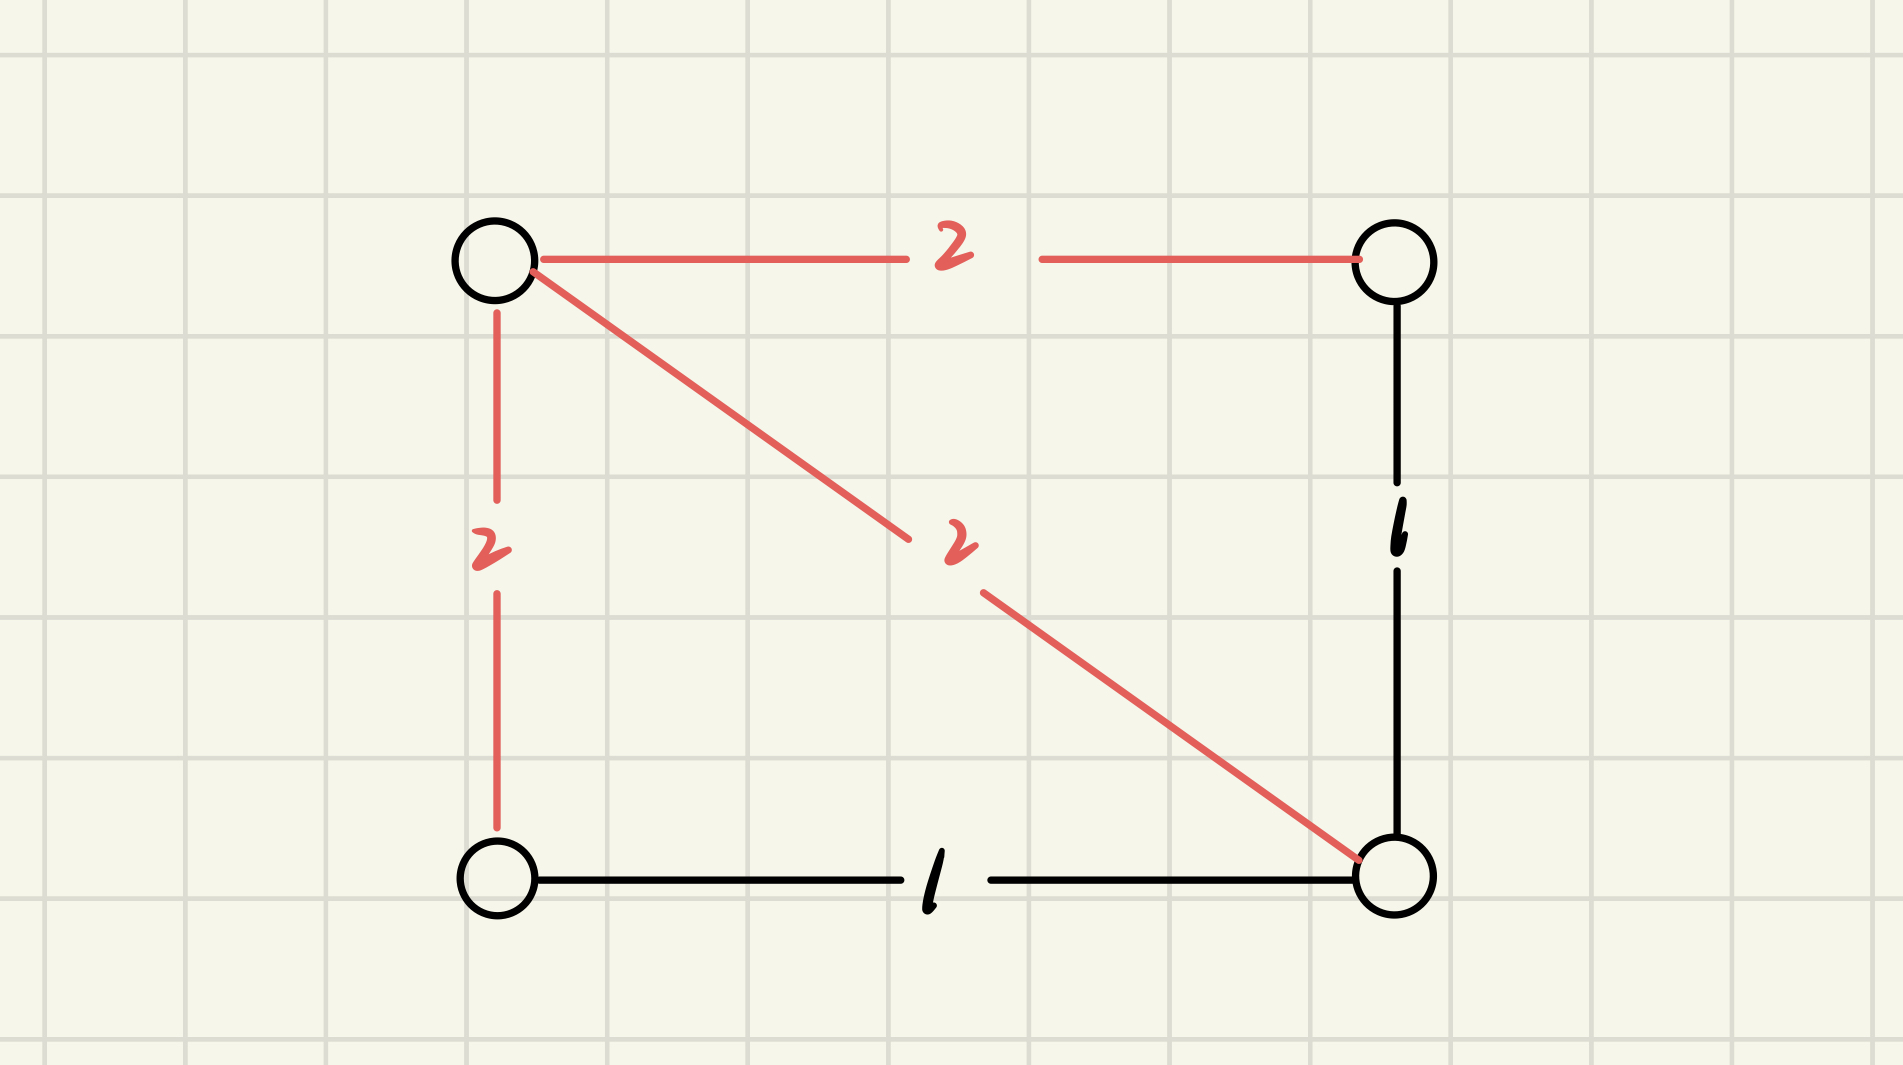
\includegraphics[width=0.75\textwidth]{hw4.jpg}}{No Figure Yet}
		\caption{BST graph of part(b)} 
	\end{figure}
	
\end{solution}
	
 \end{fun}


\end{document}





